% GNUPLOT: LaTeX picture with Postscript
\begingroup
  \makeatletter
  \providecommand\color[2][]{%
    \GenericError{(gnuplot) \space\space\space\@spaces}{%
      Package color not loaded in conjunction with
      terminal option `colourtext'%
    }{See the gnuplot documentation for explanation.%
    }{Either use 'blacktext' in gnuplot or load the package
      color.sty in LaTeX.}%
    \renewcommand\color[2][]{}%
  }%
  \providecommand\includegraphics[2][]{%
    \GenericError{(gnuplot) \space\space\space\@spaces}{%
      Package graphicx or graphics not loaded%
    }{See the gnuplot documentation for explanation.%
    }{The gnuplot epslatex terminal needs graphicx.sty or graphics.sty.}%
    \renewcommand\includegraphics[2][]{}%
  }%
  \providecommand\rotatebox[2]{#2}%
  \@ifundefined{ifGPcolor}{%
    \newif\ifGPcolor
    \GPcolortrue
  }{}%
  \@ifundefined{ifGPblacktext}{%
    \newif\ifGPblacktext
    \GPblacktexttrue
  }{}%
  % define a \g@addto@macro without @ in the name:
  \let\gplgaddtomacro\g@addto@macro
  % define empty templates for all commands taking text:
  \gdef\gplbacktext{}%
  \gdef\gplfronttext{}%
  \makeatother
  \ifGPblacktext
    % no textcolor at all
    \def\colorrgb#1{}%
    \def\colorgray#1{}%
  \else
    % gray or color?
    \ifGPcolor
      \def\colorrgb#1{\color[rgb]{#1}}%
      \def\colorgray#1{\color[gray]{#1}}%
      \expandafter\def\csname LTw\endcsname{\color{white}}%
      \expandafter\def\csname LTb\endcsname{\color{black}}%
      \expandafter\def\csname LTa\endcsname{\color{black}}%
      \expandafter\def\csname LT0\endcsname{\color[rgb]{1,0,0}}%
      \expandafter\def\csname LT1\endcsname{\color[rgb]{0,1,0}}%
      \expandafter\def\csname LT2\endcsname{\color[rgb]{0,0,1}}%
      \expandafter\def\csname LT3\endcsname{\color[rgb]{1,0,1}}%
      \expandafter\def\csname LT4\endcsname{\color[rgb]{0,1,1}}%
      \expandafter\def\csname LT5\endcsname{\color[rgb]{1,1,0}}%
      \expandafter\def\csname LT6\endcsname{\color[rgb]{0,0,0}}%
      \expandafter\def\csname LT7\endcsname{\color[rgb]{1,0.3,0}}%
      \expandafter\def\csname LT8\endcsname{\color[rgb]{0.5,0.5,0.5}}%
    \else
      % gray
      \def\colorrgb#1{\color{black}}%
      \def\colorgray#1{\color[gray]{#1}}%
      \expandafter\def\csname LTw\endcsname{\color{white}}%
      \expandafter\def\csname LTb\endcsname{\color{black}}%
      \expandafter\def\csname LTa\endcsname{\color{black}}%
      \expandafter\def\csname LT0\endcsname{\color{black}}%
      \expandafter\def\csname LT1\endcsname{\color{black}}%
      \expandafter\def\csname LT2\endcsname{\color{black}}%
      \expandafter\def\csname LT3\endcsname{\color{black}}%
      \expandafter\def\csname LT4\endcsname{\color{black}}%
      \expandafter\def\csname LT5\endcsname{\color{black}}%
      \expandafter\def\csname LT6\endcsname{\color{black}}%
      \expandafter\def\csname LT7\endcsname{\color{black}}%
      \expandafter\def\csname LT8\endcsname{\color{black}}%
    \fi
  \fi
    \setlength{\unitlength}{0.0500bp}%
    \ifx\gptboxheight\undefined%
      \newlength{\gptboxheight}%
      \newlength{\gptboxwidth}%
      \newsavebox{\gptboxtext}%
    \fi%
    \setlength{\fboxrule}{0.5pt}%
    \setlength{\fboxsep}{1pt}%
\begin{picture}(8640.00,10080.00)%
      \csname LTb\endcsname%%
      \put(4320,9894){\makebox(0,0){\strut{}Hagedorn (transmitted)wavepacket}}%
    \gplgaddtomacro\gplbacktext{%
      \colorrgb{0.50,0.50,0.50}%%
      \put(561,7583){\makebox(0,0)[r]{\strut{}$-0.2$}}%
      \colorrgb{0.50,0.50,0.50}%%
      \put(561,7845){\makebox(0,0)[r]{\strut{}$0$}}%
      \colorrgb{0.50,0.50,0.50}%%
      \put(561,8106){\makebox(0,0)[r]{\strut{}$0.2$}}%
      \colorrgb{0.50,0.50,0.50}%%
      \put(561,8368){\makebox(0,0)[r]{\strut{}$0.4$}}%
      \colorrgb{0.50,0.50,0.50}%%
      \put(561,8630){\makebox(0,0)[r]{\strut{}$0.6$}}%
      \colorrgb{0.50,0.50,0.50}%%
      \put(561,8891){\makebox(0,0)[r]{\strut{}$0.8$}}%
      \colorrgb{0.50,0.50,0.50}%%
      \put(561,9153){\makebox(0,0)[r]{\strut{}$1$}}%
      \colorrgb{0.50,0.50,0.50}%%
      \put(561,9414){\makebox(0,0)[r]{\strut{}$1.2$}}%
      \colorrgb{0.50,0.50,0.50}%%
      \put(561,9676){\makebox(0,0)[r]{\strut{}$1.4$}}%
      \colorrgb{0.50,0.50,0.50}%%
      \put(663,7397){\makebox(0,0){\strut{}}}%
      \colorrgb{0.50,0.50,0.50}%%
      \put(1082,7397){\makebox(0,0){\strut{}}}%
      \colorrgb{0.50,0.50,0.50}%%
      \put(1501,7397){\makebox(0,0){\strut{}}}%
      \colorrgb{0.50,0.50,0.50}%%
      \put(1919,7397){\makebox(0,0){\strut{}}}%
      \colorrgb{0.50,0.50,0.50}%%
      \put(2338,7397){\makebox(0,0){\strut{}}}%
      \colorrgb{0.50,0.50,0.50}%%
      \put(2757,7397){\makebox(0,0){\strut{}}}%
      \colorrgb{0.50,0.50,0.50}%%
      \put(3176,7397){\makebox(0,0){\strut{}}}%
      \colorrgb{0.50,0.50,0.50}%%
      \put(3594,7397){\makebox(0,0){\strut{}}}%
      \colorrgb{0.50,0.50,0.50}%%
      \put(4013,7397){\makebox(0,0){\strut{}}}%
    }%
    \gplgaddtomacro\gplfronttext{%
      \csname LTb\endcsname%%
      \put(3225,9462){\makebox(0,0)[r]{\strut{}$\hat{\varphi}^+_{0}$}}%
      \csname LTb\endcsname%%
      \put(3225,9183){\makebox(0,0)[r]{\strut{}$\hat{\varphi}^-_{0}$}}%
    }%
    \gplgaddtomacro\gplbacktext{%
      \colorrgb{0.50,0.50,0.50}%%
      \put(4881,7583){\makebox(0,0)[r]{\strut{}$-0.2$}}%
      \colorrgb{0.50,0.50,0.50}%%
      \put(4881,7845){\makebox(0,0)[r]{\strut{}$0$}}%
      \colorrgb{0.50,0.50,0.50}%%
      \put(4881,8106){\makebox(0,0)[r]{\strut{}$0.2$}}%
      \colorrgb{0.50,0.50,0.50}%%
      \put(4881,8368){\makebox(0,0)[r]{\strut{}$0.4$}}%
      \colorrgb{0.50,0.50,0.50}%%
      \put(4881,8630){\makebox(0,0)[r]{\strut{}$0.6$}}%
      \colorrgb{0.50,0.50,0.50}%%
      \put(4881,8891){\makebox(0,0)[r]{\strut{}$0.8$}}%
      \colorrgb{0.50,0.50,0.50}%%
      \put(4881,9153){\makebox(0,0)[r]{\strut{}$1$}}%
      \colorrgb{0.50,0.50,0.50}%%
      \put(4881,9414){\makebox(0,0)[r]{\strut{}$1.2$}}%
      \colorrgb{0.50,0.50,0.50}%%
      \put(4881,9676){\makebox(0,0)[r]{\strut{}$1.4$}}%
      \colorrgb{0.50,0.50,0.50}%%
      \put(4983,7397){\makebox(0,0){\strut{}}}%
      \colorrgb{0.50,0.50,0.50}%%
      \put(5402,7397){\makebox(0,0){\strut{}}}%
      \colorrgb{0.50,0.50,0.50}%%
      \put(5821,7397){\makebox(0,0){\strut{}}}%
      \colorrgb{0.50,0.50,0.50}%%
      \put(6239,7397){\makebox(0,0){\strut{}}}%
      \colorrgb{0.50,0.50,0.50}%%
      \put(6658,7397){\makebox(0,0){\strut{}}}%
      \colorrgb{0.50,0.50,0.50}%%
      \put(7077,7397){\makebox(0,0){\strut{}}}%
      \colorrgb{0.50,0.50,0.50}%%
      \put(7496,7397){\makebox(0,0){\strut{}}}%
      \colorrgb{0.50,0.50,0.50}%%
      \put(7914,7397){\makebox(0,0){\strut{}}}%
      \colorrgb{0.50,0.50,0.50}%%
      \put(8333,7397){\makebox(0,0){\strut{}}}%
    }%
    \gplgaddtomacro\gplfronttext{%
      \csname LTb\endcsname%%
      \put(7545,9462){\makebox(0,0)[r]{\strut{}$\hat{\varphi}^+_{0}$}}%
      \csname LTb\endcsname%%
      \put(7545,9183){\makebox(0,0)[r]{\strut{}$\hat{\varphi}^-_{0}$}}%
    }%
    \gplgaddtomacro\gplbacktext{%
      \colorrgb{0.50,0.50,0.50}%%
      \put(561,5117){\makebox(0,0)[r]{\strut{}$-1.5$}}%
      \colorrgb{0.50,0.50,0.50}%%
      \put(561,5466){\makebox(0,0)[r]{\strut{}$-1$}}%
      \colorrgb{0.50,0.50,0.50}%%
      \put(561,5815){\makebox(0,0)[r]{\strut{}$-0.5$}}%
      \colorrgb{0.50,0.50,0.50}%%
      \put(561,6164){\makebox(0,0)[r]{\strut{}$0$}}%
      \colorrgb{0.50,0.50,0.50}%%
      \put(561,6513){\makebox(0,0)[r]{\strut{}$0.5$}}%
      \colorrgb{0.50,0.50,0.50}%%
      \put(561,6862){\makebox(0,0)[r]{\strut{}$1$}}%
      \colorrgb{0.50,0.50,0.50}%%
      \put(561,7211){\makebox(0,0)[r]{\strut{}$1.5$}}%
      \colorrgb{0.50,0.50,0.50}%%
      \put(663,4931){\makebox(0,0){\strut{}}}%
      \colorrgb{0.50,0.50,0.50}%%
      \put(1082,4931){\makebox(0,0){\strut{}}}%
      \colorrgb{0.50,0.50,0.50}%%
      \put(1501,4931){\makebox(0,0){\strut{}}}%
      \colorrgb{0.50,0.50,0.50}%%
      \put(1919,4931){\makebox(0,0){\strut{}}}%
      \colorrgb{0.50,0.50,0.50}%%
      \put(2338,4931){\makebox(0,0){\strut{}}}%
      \colorrgb{0.50,0.50,0.50}%%
      \put(2757,4931){\makebox(0,0){\strut{}}}%
      \colorrgb{0.50,0.50,0.50}%%
      \put(3176,4931){\makebox(0,0){\strut{}}}%
      \colorrgb{0.50,0.50,0.50}%%
      \put(3594,4931){\makebox(0,0){\strut{}}}%
      \colorrgb{0.50,0.50,0.50}%%
      \put(4013,4931){\makebox(0,0){\strut{}}}%
    }%
    \gplgaddtomacro\gplfronttext{%
      \csname LTb\endcsname%%
      \put(3225,6997){\makebox(0,0)[r]{\strut{}$\hat{\varphi}^+_{1}$}}%
      \csname LTb\endcsname%%
      \put(3225,6718){\makebox(0,0)[r]{\strut{}$\hat{\varphi}^-_{1}$}}%
    }%
    \gplgaddtomacro\gplbacktext{%
      \colorrgb{0.50,0.50,0.50}%%
      \put(4881,5117){\makebox(0,0)[r]{\strut{}$-1.5$}}%
      \colorrgb{0.50,0.50,0.50}%%
      \put(4881,5466){\makebox(0,0)[r]{\strut{}$-1$}}%
      \colorrgb{0.50,0.50,0.50}%%
      \put(4881,5815){\makebox(0,0)[r]{\strut{}$-0.5$}}%
      \colorrgb{0.50,0.50,0.50}%%
      \put(4881,6164){\makebox(0,0)[r]{\strut{}$0$}}%
      \colorrgb{0.50,0.50,0.50}%%
      \put(4881,6513){\makebox(0,0)[r]{\strut{}$0.5$}}%
      \colorrgb{0.50,0.50,0.50}%%
      \put(4881,6862){\makebox(0,0)[r]{\strut{}$1$}}%
      \colorrgb{0.50,0.50,0.50}%%
      \put(4881,7211){\makebox(0,0)[r]{\strut{}$1.5$}}%
      \colorrgb{0.50,0.50,0.50}%%
      \put(4983,4931){\makebox(0,0){\strut{}}}%
      \colorrgb{0.50,0.50,0.50}%%
      \put(5402,4931){\makebox(0,0){\strut{}}}%
      \colorrgb{0.50,0.50,0.50}%%
      \put(5821,4931){\makebox(0,0){\strut{}}}%
      \colorrgb{0.50,0.50,0.50}%%
      \put(6239,4931){\makebox(0,0){\strut{}}}%
      \colorrgb{0.50,0.50,0.50}%%
      \put(6658,4931){\makebox(0,0){\strut{}}}%
      \colorrgb{0.50,0.50,0.50}%%
      \put(7077,4931){\makebox(0,0){\strut{}}}%
      \colorrgb{0.50,0.50,0.50}%%
      \put(7496,4931){\makebox(0,0){\strut{}}}%
      \colorrgb{0.50,0.50,0.50}%%
      \put(7914,4931){\makebox(0,0){\strut{}}}%
      \colorrgb{0.50,0.50,0.50}%%
      \put(8333,4931){\makebox(0,0){\strut{}}}%
    }%
    \gplgaddtomacro\gplfronttext{%
      \csname LTb\endcsname%%
      \put(7545,6997){\makebox(0,0)[r]{\strut{}$\hat{\varphi}^+_{1}$}}%
      \csname LTb\endcsname%%
      \put(7545,6718){\makebox(0,0)[r]{\strut{}$\hat{\varphi}^-_{1}$}}%
    }%
    \gplgaddtomacro\gplbacktext{%
      \colorrgb{0.50,0.50,0.50}%%
      \put(561,2651){\makebox(0,0)[r]{\strut{}$-1.5$}}%
      \colorrgb{0.50,0.50,0.50}%%
      \put(561,3000){\makebox(0,0)[r]{\strut{}$-1$}}%
      \colorrgb{0.50,0.50,0.50}%%
      \put(561,3349){\makebox(0,0)[r]{\strut{}$-0.5$}}%
      \colorrgb{0.50,0.50,0.50}%%
      \put(561,3698){\makebox(0,0)[r]{\strut{}$0$}}%
      \colorrgb{0.50,0.50,0.50}%%
      \put(561,4047){\makebox(0,0)[r]{\strut{}$0.5$}}%
      \colorrgb{0.50,0.50,0.50}%%
      \put(561,4396){\makebox(0,0)[r]{\strut{}$1$}}%
      \colorrgb{0.50,0.50,0.50}%%
      \put(561,4745){\makebox(0,0)[r]{\strut{}$1.5$}}%
      \colorrgb{0.50,0.50,0.50}%%
      \put(663,2465){\makebox(0,0){\strut{}}}%
      \colorrgb{0.50,0.50,0.50}%%
      \put(1082,2465){\makebox(0,0){\strut{}}}%
      \colorrgb{0.50,0.50,0.50}%%
      \put(1501,2465){\makebox(0,0){\strut{}}}%
      \colorrgb{0.50,0.50,0.50}%%
      \put(1919,2465){\makebox(0,0){\strut{}}}%
      \colorrgb{0.50,0.50,0.50}%%
      \put(2338,2465){\makebox(0,0){\strut{}}}%
      \colorrgb{0.50,0.50,0.50}%%
      \put(2757,2465){\makebox(0,0){\strut{}}}%
      \colorrgb{0.50,0.50,0.50}%%
      \put(3176,2465){\makebox(0,0){\strut{}}}%
      \colorrgb{0.50,0.50,0.50}%%
      \put(3594,2465){\makebox(0,0){\strut{}}}%
      \colorrgb{0.50,0.50,0.50}%%
      \put(4013,2465){\makebox(0,0){\strut{}}}%
    }%
    \gplgaddtomacro\gplfronttext{%
      \csname LTb\endcsname%%
      \put(3225,4531){\makebox(0,0)[r]{\strut{}$\hat{\varphi}^+_{3}$}}%
      \csname LTb\endcsname%%
      \put(3225,4252){\makebox(0,0)[r]{\strut{}$\hat{\varphi}^-_{3}$}}%
    }%
    \gplgaddtomacro\gplbacktext{%
      \colorrgb{0.50,0.50,0.50}%%
      \put(4881,2651){\makebox(0,0)[r]{\strut{}$-1.5$}}%
      \colorrgb{0.50,0.50,0.50}%%
      \put(4881,3000){\makebox(0,0)[r]{\strut{}$-1$}}%
      \colorrgb{0.50,0.50,0.50}%%
      \put(4881,3349){\makebox(0,0)[r]{\strut{}$-0.5$}}%
      \colorrgb{0.50,0.50,0.50}%%
      \put(4881,3698){\makebox(0,0)[r]{\strut{}$0$}}%
      \colorrgb{0.50,0.50,0.50}%%
      \put(4881,4047){\makebox(0,0)[r]{\strut{}$0.5$}}%
      \colorrgb{0.50,0.50,0.50}%%
      \put(4881,4396){\makebox(0,0)[r]{\strut{}$1$}}%
      \colorrgb{0.50,0.50,0.50}%%
      \put(4881,4745){\makebox(0,0)[r]{\strut{}$1.5$}}%
      \colorrgb{0.50,0.50,0.50}%%
      \put(4983,2465){\makebox(0,0){\strut{}}}%
      \colorrgb{0.50,0.50,0.50}%%
      \put(5402,2465){\makebox(0,0){\strut{}}}%
      \colorrgb{0.50,0.50,0.50}%%
      \put(5821,2465){\makebox(0,0){\strut{}}}%
      \colorrgb{0.50,0.50,0.50}%%
      \put(6239,2465){\makebox(0,0){\strut{}}}%
      \colorrgb{0.50,0.50,0.50}%%
      \put(6658,2465){\makebox(0,0){\strut{}}}%
      \colorrgb{0.50,0.50,0.50}%%
      \put(7077,2465){\makebox(0,0){\strut{}}}%
      \colorrgb{0.50,0.50,0.50}%%
      \put(7496,2465){\makebox(0,0){\strut{}}}%
      \colorrgb{0.50,0.50,0.50}%%
      \put(7914,2465){\makebox(0,0){\strut{}}}%
      \colorrgb{0.50,0.50,0.50}%%
      \put(8333,2465){\makebox(0,0){\strut{}}}%
    }%
    \gplgaddtomacro\gplfronttext{%
      \csname LTb\endcsname%%
      \put(7545,4531){\makebox(0,0)[r]{\strut{}$\hat{\varphi}^+_{3}$}}%
      \csname LTb\endcsname%%
      \put(7545,4252){\makebox(0,0)[r]{\strut{}$\hat{\varphi}^-_{3}$}}%
    }%
    \gplgaddtomacro\gplbacktext{%
      \colorrgb{0.50,0.50,0.50}%%
      \put(561,372){\makebox(0,0)[r]{\strut{}$-0.8$}}%
      \colorrgb{0.50,0.50,0.50}%%
      \put(561,584){\makebox(0,0)[r]{\strut{}$-0.6$}}%
      \colorrgb{0.50,0.50,0.50}%%
      \put(561,796){\makebox(0,0)[r]{\strut{}$-0.4$}}%
      \colorrgb{0.50,0.50,0.50}%%
      \put(561,1008){\makebox(0,0)[r]{\strut{}$-0.2$}}%
      \colorrgb{0.50,0.50,0.50}%%
      \put(561,1220){\makebox(0,0)[r]{\strut{}$0$}}%
      \colorrgb{0.50,0.50,0.50}%%
      \put(561,1432){\makebox(0,0)[r]{\strut{}$0.2$}}%
      \colorrgb{0.50,0.50,0.50}%%
      \put(561,1644){\makebox(0,0)[r]{\strut{}$0.4$}}%
      \colorrgb{0.50,0.50,0.50}%%
      \put(561,1856){\makebox(0,0)[r]{\strut{}$0.6$}}%
      \colorrgb{0.50,0.50,0.50}%%
      \put(561,2068){\makebox(0,0)[r]{\strut{}$0.8$}}%
      \colorrgb{0.50,0.50,0.50}%%
      \put(561,2280){\makebox(0,0)[r]{\strut{}$1$}}%
      \colorrgb{0.50,0.50,0.50}%%
      \put(663,186){\makebox(0,0){\strut{}2.0}}%
      \colorrgb{0.50,0.50,0.50}%%
      \put(1082,186){\makebox(0,0){\strut{}2.5}}%
      \colorrgb{0.50,0.50,0.50}%%
      \put(1501,186){\makebox(0,0){\strut{}3.0}}%
      \colorrgb{0.50,0.50,0.50}%%
      \put(1919,186){\makebox(0,0){\strut{}3.5}}%
      \colorrgb{0.50,0.50,0.50}%%
      \put(2338,186){\makebox(0,0){\strut{}4.0}}%
      \colorrgb{0.50,0.50,0.50}%%
      \put(2757,186){\makebox(0,0){\strut{}4.5}}%
      \colorrgb{0.50,0.50,0.50}%%
      \put(3176,186){\makebox(0,0){\strut{}5.0}}%
      \colorrgb{0.50,0.50,0.50}%%
      \put(3594,186){\makebox(0,0){\strut{}5.5}}%
      \colorrgb{0.50,0.50,0.50}%%
      \put(4013,186){\makebox(0,0){\strut{}6.0}}%
    }%
    \gplgaddtomacro\gplfronttext{%
      \csname LTb\endcsname%%
      \put(3225,2066){\makebox(0,0)[r]{\strut{}$\hat{\varphi}^+_{10}$}}%
      \csname LTb\endcsname%%
      \put(3225,1787){\makebox(0,0)[r]{\strut{}$\hat{\varphi}^-_{10}$}}%
    }%
    \gplgaddtomacro\gplbacktext{%
      \colorrgb{0.50,0.50,0.50}%%
      \put(4881,372){\makebox(0,0)[r]{\strut{}$-0.8$}}%
      \colorrgb{0.50,0.50,0.50}%%
      \put(4881,584){\makebox(0,0)[r]{\strut{}$-0.6$}}%
      \colorrgb{0.50,0.50,0.50}%%
      \put(4881,796){\makebox(0,0)[r]{\strut{}$-0.4$}}%
      \colorrgb{0.50,0.50,0.50}%%
      \put(4881,1008){\makebox(0,0)[r]{\strut{}$-0.2$}}%
      \colorrgb{0.50,0.50,0.50}%%
      \put(4881,1220){\makebox(0,0)[r]{\strut{}$0$}}%
      \colorrgb{0.50,0.50,0.50}%%
      \put(4881,1432){\makebox(0,0)[r]{\strut{}$0.2$}}%
      \colorrgb{0.50,0.50,0.50}%%
      \put(4881,1644){\makebox(0,0)[r]{\strut{}$0.4$}}%
      \colorrgb{0.50,0.50,0.50}%%
      \put(4881,1856){\makebox(0,0)[r]{\strut{}$0.6$}}%
      \colorrgb{0.50,0.50,0.50}%%
      \put(4881,2068){\makebox(0,0)[r]{\strut{}$0.8$}}%
      \colorrgb{0.50,0.50,0.50}%%
      \put(4881,2280){\makebox(0,0)[r]{\strut{}$1$}}%
      \colorrgb{0.50,0.50,0.50}%%
      \put(4983,186){\makebox(0,0){\strut{}2.0}}%
      \colorrgb{0.50,0.50,0.50}%%
      \put(5402,186){\makebox(0,0){\strut{}2.5}}%
      \colorrgb{0.50,0.50,0.50}%%
      \put(5821,186){\makebox(0,0){\strut{}3.0}}%
      \colorrgb{0.50,0.50,0.50}%%
      \put(6239,186){\makebox(0,0){\strut{}3.5}}%
      \colorrgb{0.50,0.50,0.50}%%
      \put(6658,186){\makebox(0,0){\strut{}4.0}}%
      \colorrgb{0.50,0.50,0.50}%%
      \put(7077,186){\makebox(0,0){\strut{}4.5}}%
      \colorrgb{0.50,0.50,0.50}%%
      \put(7496,186){\makebox(0,0){\strut{}5.0}}%
      \colorrgb{0.50,0.50,0.50}%%
      \put(7914,186){\makebox(0,0){\strut{}5.5}}%
      \colorrgb{0.50,0.50,0.50}%%
      \put(8333,186){\makebox(0,0){\strut{}6.0}}%
    }%
    \gplgaddtomacro\gplfronttext{%
      \csname LTb\endcsname%%
      \put(7545,2066){\makebox(0,0)[r]{\strut{}$\hat{\varphi}^+_{10}$}}%
      \csname LTb\endcsname%%
      \put(7545,1787){\makebox(0,0)[r]{\strut{}$\hat{\varphi}^-_{10}$}}%
    }%
    \gplbacktext
    \put(0,0){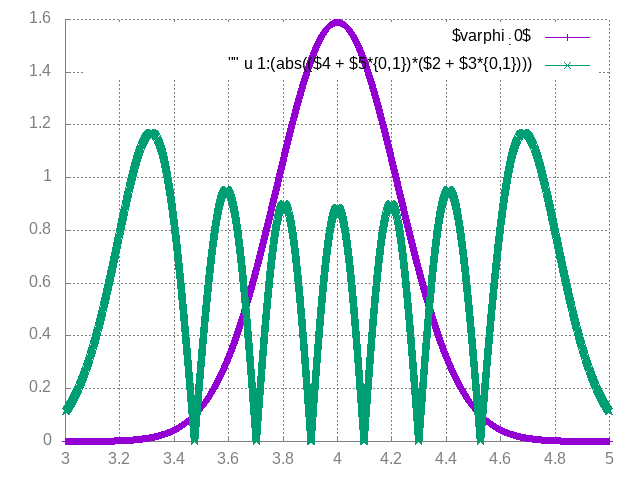
\includegraphics{/home/s1992054/NAQMD/src/Hagedorn/plots/hagedorn_gaussian}}%
    \gplfronttext
  \end{picture}%
\endgroup
